\documentclass[12pt]{article}
\usepackage[utf8]{inputenc}
\usepackage{geometry}
\usepackage{graphicx}
\usepackage{longtable}
\usepackage{url}
\usepackage{amsmath}
\usepackage[alf]{abntex2cite} % Citações ABNT 2
\usepackage{setspace} % Espaçamento entre linhas
\usepackage{float} 
\usepackage{xcolor}
\geometry{a4paper, left=3cm, right=2cm, top=3cm, bottom=2cm}


\begin{document}
\onehalfspacing
% Capa incorporada
\begin{titlepage}
    \centering
    \vspace*{2cm}
    {\Large Centro Federal de Educação Tecnológica de Minas Gerais}\\[0.7cm]
    {\large Programa de Pós-Graduação em Computação Aplicada}\\[0.5cm]
    {\large Doutorado em Computação Aplicada}\\[2.5cm]
    {\LARGE \textbf{Problema do Caixeiro Chinês}}\\[2.5cm]
    {\large Leonardo Vieira Guimarães}\\[5.5cm]
    {\large Belo Horizonte}\\[0.3cm]
    {\large Dezembro de 2025}
    \vspace*{2cm}
\end{titlepage}
\setcounter{page}{1}

\section{Introdução}


O Problema do Caixeiro Chinês (ou Carteiro Chinês) busca encontrar um circuito fechado de menor custo que percorra todas as arestas de um grafo ao menos uma vez. Proposto por Mei-Ko Kwan em 1962, tem aplicações práticas em logística, inspeção de ruas, coleta de lixo e redes urbanas.

Este trabalho apresenta uma implementação do algoritmo para a solução ótima do problema, utilizando Python e NetworkX. Foram testadas cinco instâncias: uma de teste e quatro reais no formato .tsp (gr15.tsp, gr17.tsp, gr21.tsp, gr24.tsp), avaliando desempenho e generalidade da abordagem.

O estudo contribui para o desenvolvimento de técnicas eficientes de roteirização e otimização logística, reforçando conceitos de emparelhamento de vértices de grau ímpar, caminhos mínimos e circuitos eulerianos.

\section{Fundamentos Teóricos}

O \textbf{Problema do Caixeiro Chinês} consiste em encontrar um circuito fechado de menor custo que percorra todas as arestas de um grafo pelo menos uma vez, minimizando o total percorrido. Esse problema, também chamado de Problema do Carteiro Chinês, foi formalizado por Mei-Ko Kwan em 1962 e possui aplicações práticas em logística, inspeção de ruas, coleta de lixo e redes urbanas \cite{boaventura2002grafos,feofiloff2011introduccao}.

Para que seja possível percorrer todas as arestas de um grafo em um único circuito fechado, é necessário que o grafo seja \textbf{euleriano}. O \textit{Teorema de Euler} estabelece que um grafo conexo é euleriano se, e somente se, todos os seus vértices possuem grau par. Caso contrário, é preciso duplicar algumas arestas (eulerização) para garantir essa propriedade \cite{boaventura2002grafos}.


O algoritmo clássico para encontrar circuitos eulerianos foi proposto por Hierholzer em 1873. O método consiste em iniciar o percurso em qualquer vértice e seguir arestas não visitadas até retornar ao ponto de partida, formando um ciclo. Caso existam arestas não visitadas, o ciclo é expandido até que todas as arestas sejam percorridas. Esse procedimento é eficiente e garante a construção do circuito euleriano em grafos conexos com todos os vértices de grau par \cite{hierholzer1873}.


O pseudocódigo do algoritmo de Hierholzer, pensado para implementação em programação, pode ser descrito assim:

\begin{quote}
	\textbf{Algoritmo de Hierholzer para Circuito Euleriano}

\begin{verbatim}
Hierholzer(Grafo G):
    ciclo = lista vazia
    pilha = lista vazia
    v = vértice inicial
    pilha.push(v)
    enquanto pilha não está vazia:
        u = pilha.topo()
        se u tem arestas não visitadas:
            escolha uma aresta (u, w) não visitada
            marque (u, w) como visitada
            pilha.push(w)
        senão:
            ciclo.append(u)
            pilha.pop()
    retorne ciclo invertido
\end{verbatim}
\end{quote}

Na solução do Problema do Caixeiro Chinês, após a eulerização do grafo (emparelhamento dos vértices de grau ímpar e duplicação das arestas de menor custo), o algoritmo de Hierholzer é utilizado para encontrar o circuito euleriano de menor custo, garantindo que todas as arestas sejam percorridas ao menos uma vez. Essa abordagem é fundamental para a obtenção de soluções ótimas e eficientes em problemas de roteamento.

\section{Metodologia}

O trabalho foi desenvolvido em duas etapas principais:

\subsection{Implementação do Algoritmo}

O objetivo inicial foi implementar um algoritmo para a solução ótima do Problema do Caixeiro Chinês, utilizando Python e a biblioteca NetworkX. O desenvolvimento foi modular, contemplando:

\begin{itemize}
    \item \textbf{Caminho Mínimo}: Utilização do algoritmo de Dijkstra para encontrar os menores caminhos entre vértices de grau ímpar.
    \item \textbf{Emparelhamento}: Emparelhamento ótimo dos vértices de grau ímpar, duplicando arestas para tornar o grafo euleriano.
    \item \textbf{Circuito Euleriano}: Após a eulerização, obtenção do circuito euleriano de menor custo.
\end{itemize}

\subsection{Testes e Validação}

A segunda etapa consistiu em testar o algoritmo implementado em cinco instâncias distintas. A instância de teste foi utilizada para validar a corretude da implementação, com um grafo simples e conhecido. As quatro instâncias do AVA são as seguintes:

\begin{itemize}
    \item \textbf{gr15.tsp:} Grafo com 15 vértices, representando cidades e as distâncias explícitas entre cada par. É uma instância de porte intermediário, útil para avaliar o desempenho do algoritmo em um cenário não trivial.
    
    \item \textbf{gr17.tsp:} Grafo com 17 vértices, também com distâncias explícitas. Apresenta maior complexidade e serve para testar a escalabilidade da solução.
    
    \item \textbf{gr21.tsp:} Instância com 21 cidades, baseada em problemas clássicos de roteamento. As distâncias são fornecidas em formato de matriz triangular inferior, exigindo tratamento específico na leitura dos dados.
    
    \item \textbf{gr24.tsp:} A maior instância utilizada, com 24 vértices e distâncias explícitas entre pares de cidades. Permite avaliar o algoritmo em cenários mais próximos de aplicações reais, onde o número de vértices e arestas é significativo.
\end{itemize}

Todas as instâncias seguem o formato TSPLIB, com matriz de distâncias explícitas entre cidades. Para cada uma delas, o algoritmo gera imagens do grafo original e do circuito euleriano encontrado, além do percurso ótimo. Essas imagens e resultados ilustram o funcionamento do algoritmo e permitem comparar a qualidade das soluções obtidas em diferentes cenários.

\subsection{Métricas de Avaliação}

Para avaliar a qualidade e o desempenho da solução do Problema do Caixeiro Chinês, foram definidas as seguintes métricas:

\begin{itemize}
    \item \textbf{Dimensão (Dim)}: Número total de vértices presentes no grafo. Indica o tamanho da instância a ser processada.
    
    \item \textbf{Arestas Originais}: Quantidade total de arestas no grafo original antes da eulerização. Define a estrutura de conectividade do grafo.
    
    \item \textbf{Custo Original (C. Orig.)}: Soma dos pesos de todas as arestas do grafo original. Representa o custo mínimo teórico se fosse possível percorrer cada aresta apenas uma vez. Obtido através da fórmula: $\text{Custo Original} = \sum_{(u,v) \in E} w(u,v)$
    
    \item \textbf{Custo Final (C. Final)}: Soma dos pesos de todas as arestas no circuito euleriano, incluindo as arestas duplicadas pelo processo de emparelhamento. Representa o custo real do percurso ótimo encontrado que percorre todas as arestas e retorna ao ponto inicial.
    
    \item \textbf{Vértices de Grau Ímpar (V. Ím.)}: Número de vértices que possuem um número ímpar de arestas incidentes no grafo original. Segundo o Teorema de Handshaking, todo grafo conexo possui um número par de vértices com grau ímpar. Estes vértices precisam ser emparelhados (conectados por caminhos mínimos) para tornar o grafo euleriano, ou seja, permitir um circuito que percorra cada aresta exatamente uma vez.
    
    \item \textbf{Arestas Duplicadas (A. Dup.)}: Número de arestas que foram duplicadas (adicionadas) durante o processo de emparelhamento dos vértices de grau ímpar. Cada duplicação aumenta o custo total do percurso. O número de arestas duplicadas é determinado pela qualidade do emparelhamento ótimo.
    
    \item \textbf{Overhead}: Diferença absoluta entre o custo final e o custo original, representando o custo adicional introduzido pelo emparelhamento. Calculado como: $\text{Overhead} = \text{Custo Final} - \text{Custo Original}$. Quanto menor o overhead, melhor a qualidade da solução.
    
    \item \textbf{Overhead (\%) (O. \%)}: Overhead expresso como percentual do custo original. Permite comparar proporcionalmente o impacto da duplicação entre instâncias de diferentes tamanhos. Uma instância pequena pode ter overhead absoluto menor que uma instância grande, mas o percentual relativo pode ser maior. Calculado como: $\text{Overhead (\%)} = \frac{\text{Overhead}}{\text{Custo Original}} \times 100$.
\end{itemize}

\section{Resultados e Discussão}


Nesta seção, apresentamos os resultados obtidos a partir da implementação do algoritmo do Caixeiro Chinês, organizados conforme as instâncias analisadas:

\begin{enumerate}
    \item \textbf{Instância de teste}
    \item \textbf{Instância gr15.tsp}
    \item \textbf{Instância gr17.tsp}
    \item \textbf{Instância gr21.tsp}
    \item \textbf{Instância gr24.tsp}
\end{enumerate}

\subsection{Análise da instância de teste}

Para a validação do método, foi utilizada uma instância de teste composta por 7 vértices (a, b, c, d, e, f, g) e 12 arestas, cada uma com pesos explícitos representando as distâncias entre os vértices. A estrutura do grafo pode ser visualizada na Figura~\ref{fig:grafo_aula}.

\begin{figure}[H]
    \centering
    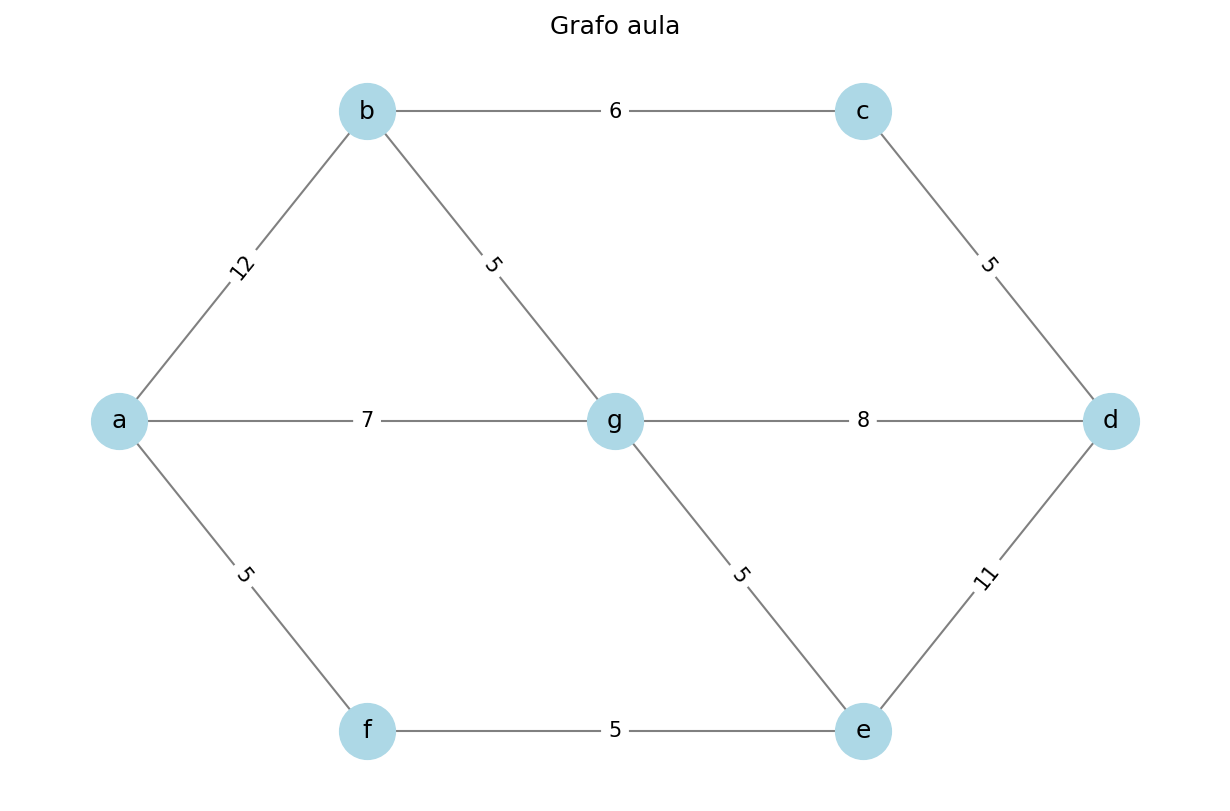
\includegraphics[width=0.6\textwidth]{./resultado/grafo_aula.png}
    \caption{Grafo original da instância de teste}
    \label{fig:grafo_aula}
\end{figure}

\textbf{Resultados obtidos:}
\begin{itemize}
    \item Dimensão (Vértices): 7
    \item Arestas Originais: 10
    \item Custo Original: 72
    \item Custo Final: 95
    \item Vértices de Grau Ímpar: 4
    \item Arestas Duplicadas: 2
    \item Overhead: 23 (31.94\%)
\end{itemize}

Após a eulerização do grafo, ou seja, a duplicação das arestas necessárias para garantir que todos os vértices tenham grau par, foi possível encontrar o circuito euleriano de menor custo. O percurso ótimo obtido está detalhado na Tabela~\ref{tab:percurso_aula} e ilustrado na Figura~\ref{fig:circuito_euleriano_aula}.

  
\begin{table}[H]
    \centering
    \scriptsize
    \begin{tabular}{|c|c|c|c|c|}
        \hline
        \multicolumn{5}{|c|}{Percurso} \\ \hline
    a -- (5) $\rightarrow$ f & f -- (5) $\rightarrow$ e & \textcolor{red}{e -- (11) $\rightarrow$ d} & \textcolor{red}{d -- (11) $\rightarrow$ e} & e -- (6) $\rightarrow$ g \\
    g -- (8) $\rightarrow$ d & d -- (5) $\rightarrow$ c & c -- (6) $\rightarrow$ b & b -- (7) $\rightarrow$ g & g -- (7) $\rightarrow$ a \\
    \textcolor{red}{a -- (12) $\rightarrow$ b} & \textcolor{red}{b -- (12) $\rightarrow$ a} &   &   &   \\
        \hline
    \end{tabular}
    \caption{Percurso ótimo encontrado para a Instância de Teste. Células em vermelho indicam arestas emparelhadas pelo algoritmo.}
    \label{tab:percurso_aula}
\end{table}



\begin{figure}[H]
    \centering
    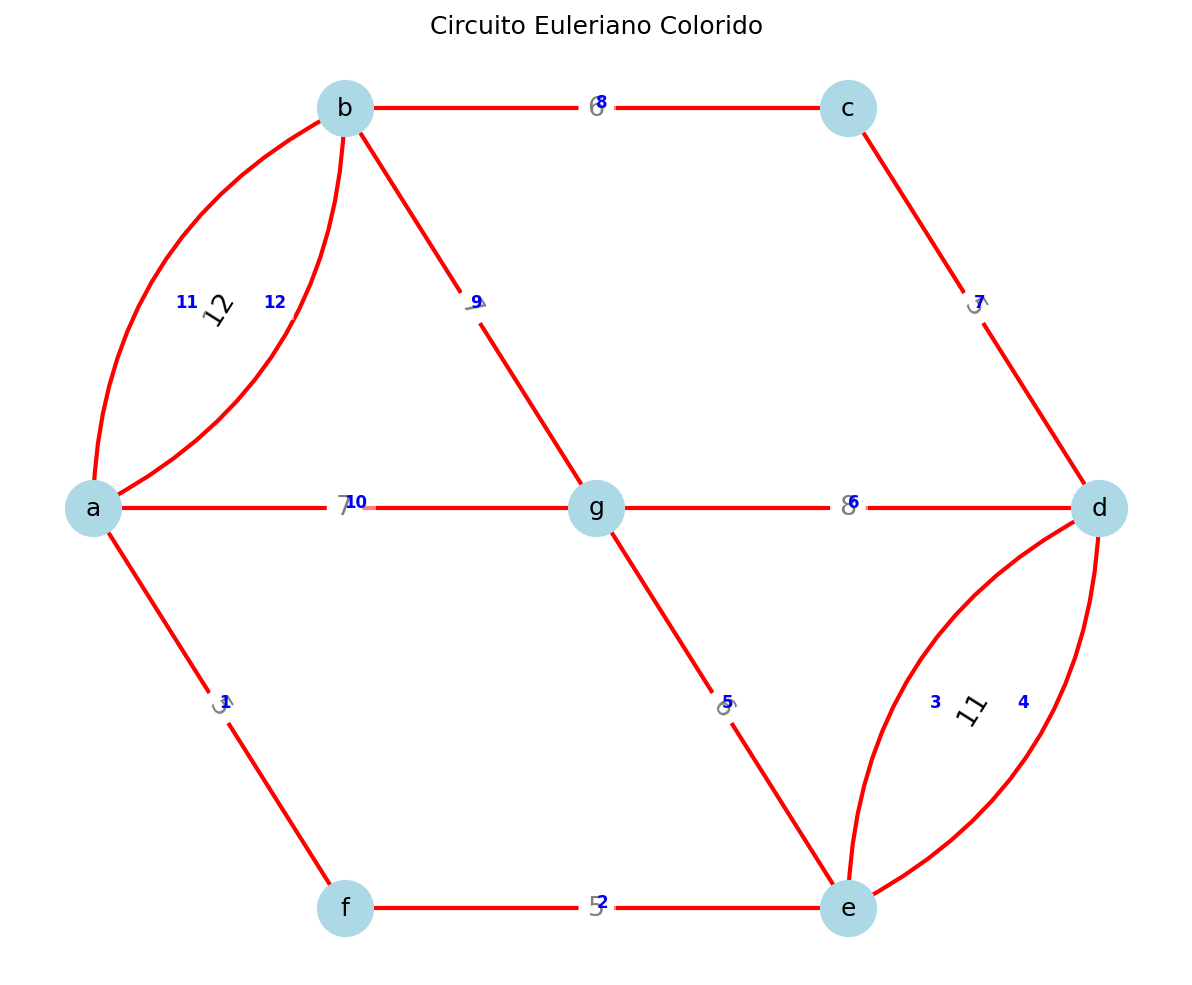
\includegraphics[width=0.6\textwidth]{./resultado/circuito_euleriano_aula.png}
    \caption{Circuito euleriano encontrado para a instância de teste}
    \label{fig:circuito_euleriano_aula}
\end{figure}

O percurso apresentado na tabela corresponde exatamente ao caminho percorrido no circuito euleriano, garantindo que todas as arestas do grafo sejam visitadas ao menos uma vez com o menor custo total possível. As imagens e a tabela permitem validar visualmente e numericamente a solução encontrada pelo algoritmo.

\subsection{Análise da instância gr15.tsp}

A instância gr15.tsp consiste em um grafo com 15 vértices, representando cidades e as distâncias explícitas entre cada par. Essa instância é útil para avaliar o desempenho do algoritmo em um cenário intermediário, com maior número de vértices e arestas em relação ao exemplo de teste.

\noindent A Figura~\ref{fig:grafo_gr15} apresenta o grafo original da instância gr15.tsp. O percurso ótimo está detalhado na Tabela~\ref{tab:percurso_gr15} e ilustrado na Figura~\ref{fig:circuito_euleriano_gr15}.

\begin{figure}[H]
    \centering
    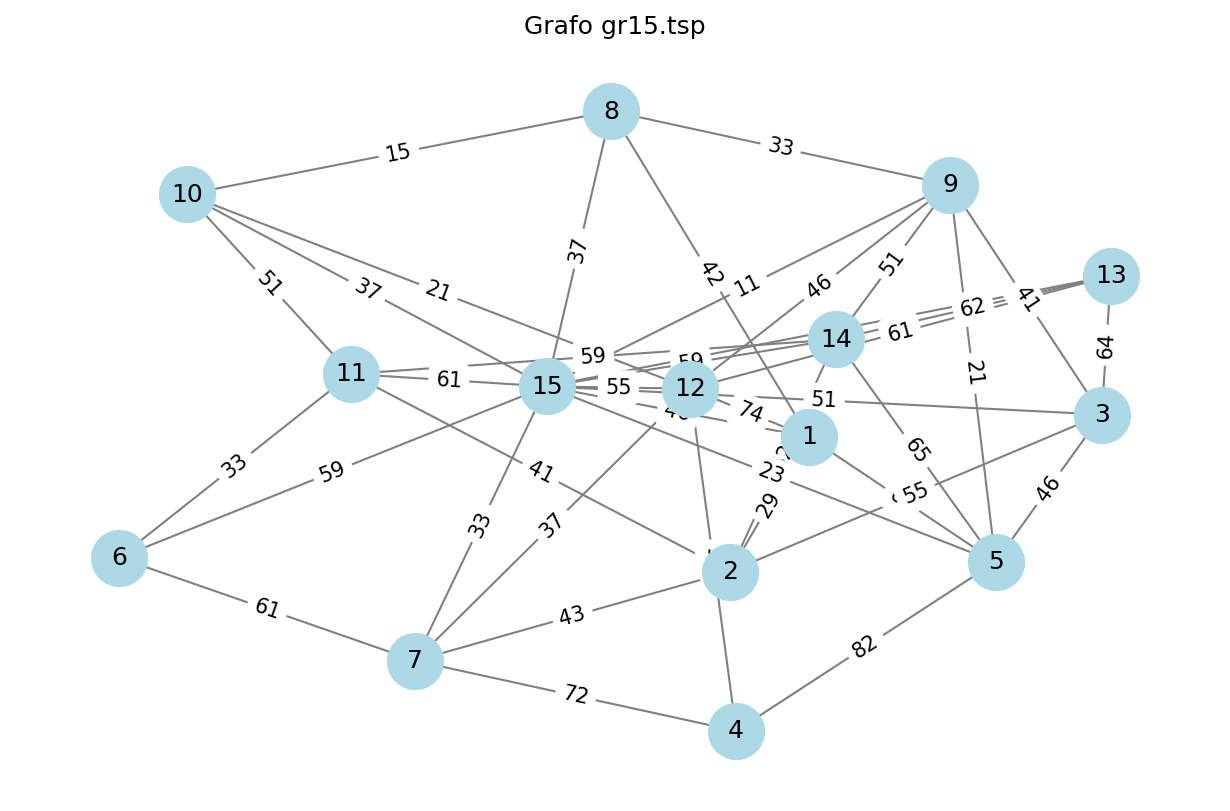
\includegraphics[width=0.6\textwidth]{./resultado/grafo_gr15.tsp.png}
    \caption{Grafo original da instância gr15.tsp}
    \label{fig:grafo_gr15}
\end{figure}

\textbf{Resultados obtidos:}
\begin{itemize}
    \item Dimensão (Vértices): 15
    \item Arestas Originais: 40
    \item Custo Original: 1871
    \item Custo Final: 2105
    \item Vértices de Grau Ímpar: 8
    \item Arestas Duplicadas: 4
    \item Overhead: 234 (12.51\%)
\end{itemize}

\begin{table}[H]
    \centering
    \scriptsize
    \begin{tabular}{|c|c|c|c|c|}
        \hline
        \multicolumn{5}{|c|}{Percurso} \\ \hline
    \textcolor{red}{1 -- (74) $\rightarrow$ 12} & 12 -- (55) $\rightarrow$ 15 & 15 -- (59) $\rightarrow$ 14 & 14 -- (62) $\rightarrow$ 13 & 13 -- (64) $\rightarrow$ 3 \\
    3 -- (41) $\rightarrow$ 9 & 9 -- (51) $\rightarrow$ 14 & 14 -- (59) $\rightarrow$ 11 & \textcolor{red}{11 -- (33) $\rightarrow$ 6} & \textcolor{red}{6 -- (33) $\rightarrow$ 11} \\
    11 -- (51) $\rightarrow$ 10 & 10 -- (37) $\rightarrow$ 15 & 15 -- (33) $\rightarrow$ 7 & \textcolor{red}{7 -- (72) $\rightarrow$ 4} & \textcolor{red}{4 -- (72) $\rightarrow$ 7} \\
    7 -- (61) $\rightarrow$ 6 & 6 -- (59) $\rightarrow$ 15 & 15 -- (23) $\rightarrow$ 13 & 13 -- (61) $\rightarrow$ 12 & 12 -- (21) $\rightarrow$ 10 \\
    10 -- (15) $\rightarrow$ 8 & 8 -- (37) $\rightarrow$ 15 & 15 -- (61) $\rightarrow$ 11 & 11 -- (41) $\rightarrow$ 2 & 2 -- (52) $\rightarrow$ 14 \\
    14 -- (65) $\rightarrow$ 5 & 5 -- (23) $\rightarrow$ 15 & 15 -- (11) $\rightarrow$ 9 & 9 -- (46) $\rightarrow$ 12 & 12 -- (51) $\rightarrow$ 4 \\
    4 -- (82) $\rightarrow$ 5 & 5 -- (21) $\rightarrow$ 9 & 9 -- (33) $\rightarrow$ 8 & 8 -- (42) $\rightarrow$ 1 & 1 -- (46) $\rightarrow$ 15 \\
    15 -- (51) $\rightarrow$ 3 & 3 -- (46) $\rightarrow$ 5 & 5 -- (68) $\rightarrow$ 1 & \textcolor{red}{1 -- (74) $\rightarrow$ 12} & 12 -- (37) $\rightarrow$ 7 \\
    7 -- (43) $\rightarrow$ 2 & \textcolor{red}{2 -- (55) $\rightarrow$ 3} & \textcolor{red}{3 -- (55) $\rightarrow$ 2} & 2 -- (29) $\rightarrow$ 1 &   \\
        \hline
    \end{tabular}
    \caption{Percurso ótimo encontrado para a Instância gr15.tsp. Células em vermelho indicam arestas emparelhadas pelo algoritmo.}
    \label{tab:percurso_gr15}
\end{table}



\begin{figure}[H]
    \centering
    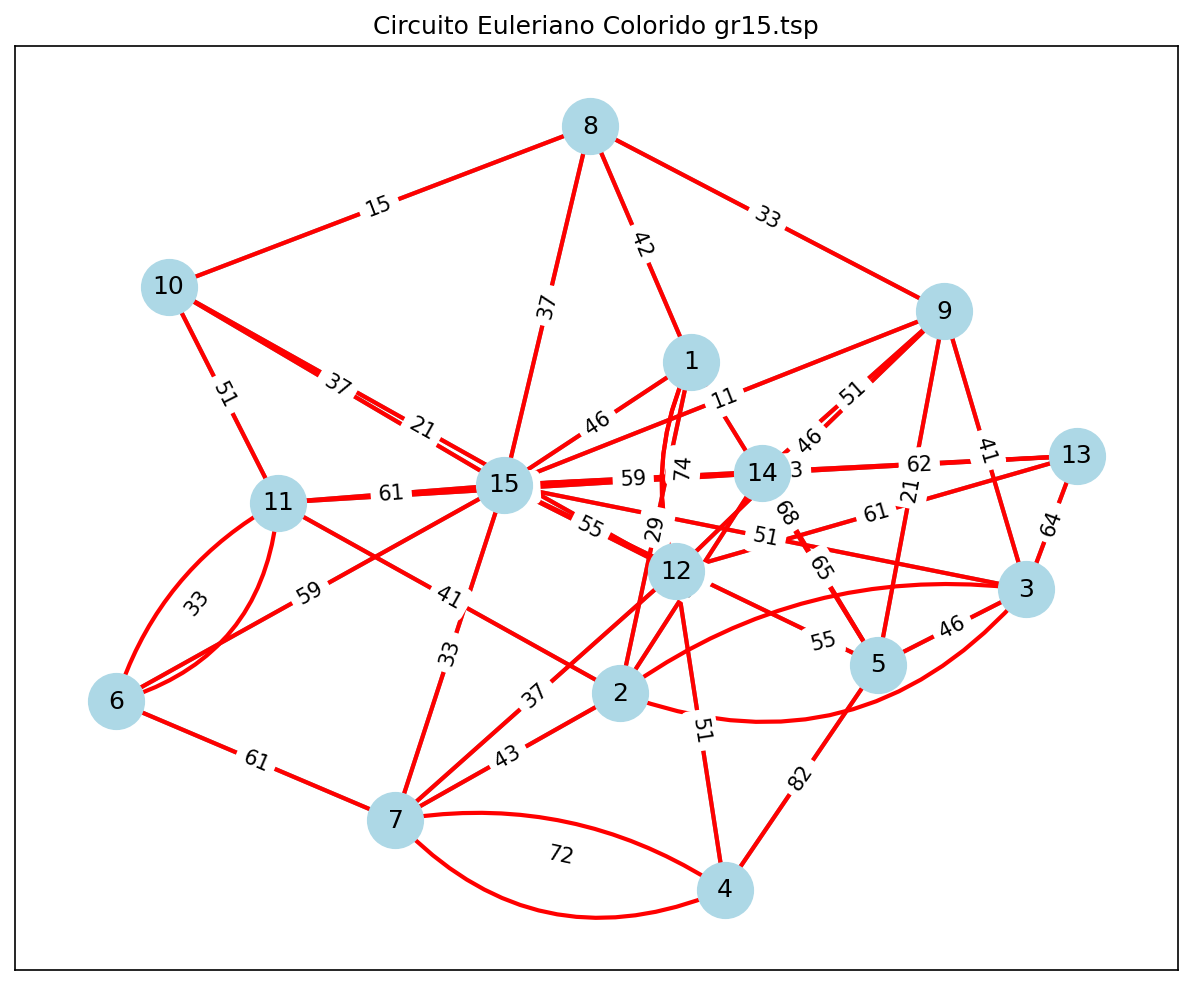
\includegraphics[width=0.6\textwidth]{./resultado/circuito_euleriano_gr15.tsp.png}
    \caption{Circuito euleriano encontrado para a instância gr15.tsp}
    \label{fig:circuito_euleriano_gr15}
\end{figure}

O percurso apresentado na tabela corresponde ao caminho percorrido no circuito euleriano da instância gr15.tsp, garantindo que todas as arestas do grafo sejam visitadas ao menos uma vez com o menor custo total possível. As imagens e a tabela permitem validar visualmente e numericamente a solução encontrada pelo algoritmo para um grafo de maior complexidade.

\subsection{Análise da instância gr17.tsp}

A instância gr17.tsp consiste em um grafo com 17 vértices, com maior complexidade e distâncias explícitas entre pares de cidades. Essa instância é útil para testar a escalabilidade da solução e avaliar o desempenho do algoritmo em cenários mais desafiadores.

\noindent A Figura~\ref{fig:grafo_gr17} apresenta o grafo original da instância gr17.tsp. O percurso ótimo está detalhado na Tabela~\ref{tab:percurso_gr17} e ilustrado na Figura~\ref{fig:circuito_euleriano_gr17}.

\begin{figure}[H]
    \centering
    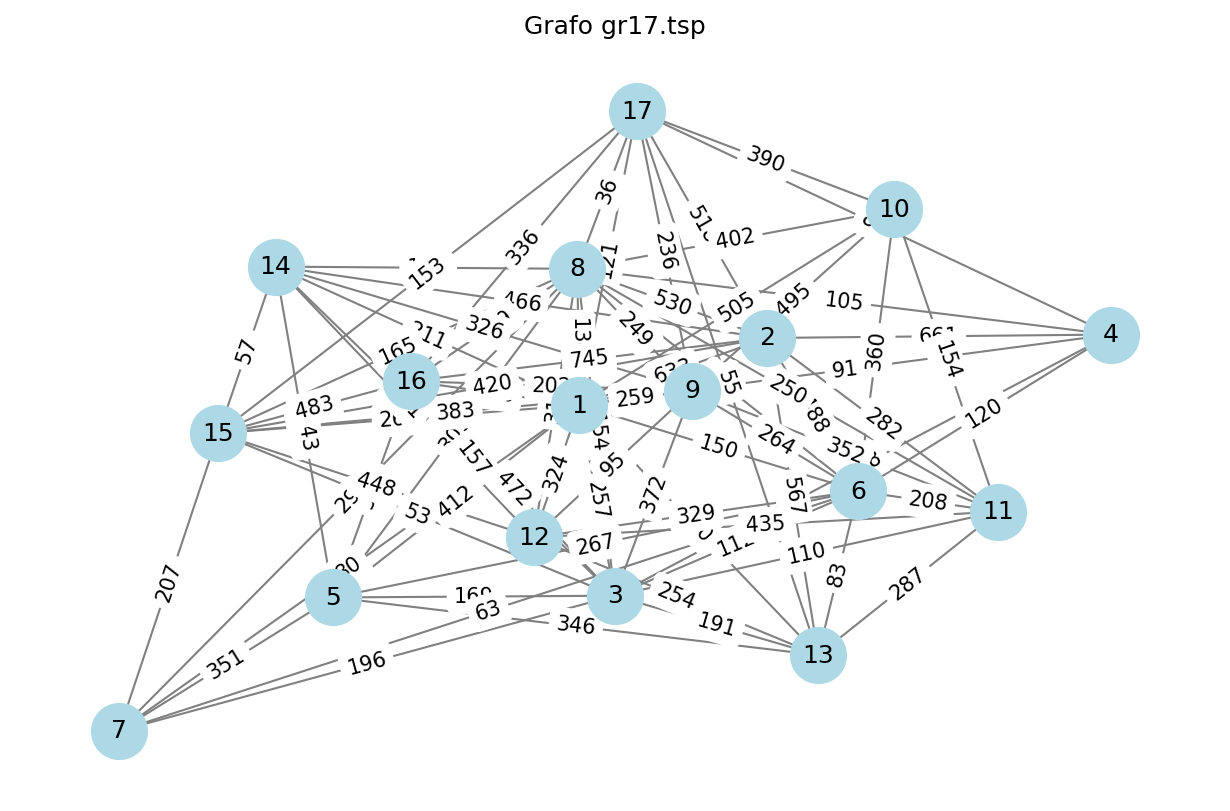
\includegraphics[width=0.6\textwidth]{./resultado/grafo_gr17.tsp.png}
    \caption{Grafo original da instância gr17.tsp}
    \label{fig:grafo_gr17}
\end{figure}

\textbf{Resultados obtidos:}
\begin{itemize}
    \item Dimensão (Vértices): 17
    \item Arestas Originais: 81
    \item Custo Original: 22061
    \item Custo Final: 22626
    \item Vértices de Grau Ímpar: 6
    \item Arestas Duplicadas: 3
    \item Overhead: 565 (2.56\%)
\end{itemize}

\begin{table}[H]
    \centering
    \scriptsize
    \begin{tabular}{|c|c|c|c|c|}
        \hline
        \multicolumn{5}{|c|}{Percurso} \\ \hline
    \textcolor{red}{1 -- (121) $\rightarrow$ 17} & 17 -- (336) $\rightarrow$ 16 & 16 -- (483) $\rightarrow$ 15 & 15 -- (57) $\rightarrow$ 14 & 14 -- (391) $\rightarrow$ 12 \\
    12 -- (448) $\rightarrow$ 15 & 15 -- (153) $\rightarrow$ 17 & 17 -- (55) $\rightarrow$ 13 & 13 -- (287) $\rightarrow$ 11 & 11 -- (435) $\rightarrow$ 12 \\
    12 -- (157) $\rightarrow$ 16 & \textcolor{red}{16 -- (349) $\rightarrow$ 8} & \textcolor{red}{8 -- (349) $\rightarrow$ 16} & 16 -- (202) $\rightarrow$ 9 & 9 -- (383) $\rightarrow$ 15 \\
    15 -- (165) $\rightarrow$ 8 & 8 -- (108) $\rightarrow$ 14 & 14 -- (326) $\rightarrow$ 9 & \textcolor{red}{9 -- (95) $\rightarrow$ 12} & \textcolor{red}{12 -- (95) $\rightarrow$ 9} \\
    9 -- (236) $\rightarrow$ 17 & 17 -- (390) $\rightarrow$ 10 & 10 -- (154) $\rightarrow$ 11 & 11 -- (250) $\rightarrow$ 8 & 8 -- (314) $\rightarrow$ 12 \\
    12 -- (254) $\rightarrow$ 13 & 13 -- (83) $\rightarrow$ 6 & 6 -- (208) $\rightarrow$ 11 & 11 -- (352) $\rightarrow$ 9 & 9 -- (495) $\rightarrow$ 10 \\
    10 -- (402) $\rightarrow$ 8 & 8 -- (36) $\rightarrow$ 17 & 17 -- (518) $\rightarrow$ 2 & 2 -- (420) $\rightarrow$ 15 & 15 -- (53) $\rightarrow$ 3 \\
    3 -- (472) $\rightarrow$ 16 & 16 -- (528) $\rightarrow$ 5 & 5 -- (243) $\rightarrow$ 14 & 14 -- (466) $\rightarrow$ 2 & 2 -- (745) $\rightarrow$ 16 \\
    16 -- (246) $\rightarrow$ 1 & 1 -- (268) $\rightarrow$ 15 & 15 -- (207) $\rightarrow$ 7 & 7 -- (29) $\rightarrow$ 8 & 8 -- (249) $\rightarrow$ 9 \\
    9 -- (264) $\rightarrow$ 6 & 6 -- (329) $\rightarrow$ 12 & 12 -- (324) $\rightarrow$ 1 & 1 -- (211) $\rightarrow$ 14 & 14 -- (74) $\rightarrow$ 3 \\
    3 -- (191) $\rightarrow$ 13 & 13 -- (346) $\rightarrow$ 5 & 5 -- (309) $\rightarrow$ 8 & 8 -- (34) $\rightarrow$ 6 & 6 -- (63) $\rightarrow$ 7 \\
    7 -- (351) $\rightarrow$ 5 & 5 -- (267) $\rightarrow$ 6 & 6 -- (360) $\rightarrow$ 10 & 10 -- (505) $\rightarrow$ 1 & 1 -- (70) $\rightarrow$ 13 \\
    13 -- (567) $\rightarrow$ 2 & 2 -- (282) $\rightarrow$ 11 & 11 -- (110) $\rightarrow$ 3 & 3 -- (372) $\rightarrow$ 9 & 9 -- (259) $\rightarrow$ 1 \\
    \textcolor{red}{1 -- (121) $\rightarrow$ 17} & 17 -- (84) $\rightarrow$ 4 & 4 -- (105) $\rightarrow$ 8 & 8 -- (154) $\rightarrow$ 3 & 3 -- (196) $\rightarrow$ 7 \\
    7 -- (80) $\rightarrow$ 1 & 1 -- (134) $\rightarrow$ 8 & 8 -- (530) $\rightarrow$ 2 & 2 -- (488) $\rightarrow$ 6 & 6 -- (112) $\rightarrow$ 3 \\
    3 -- (169) $\rightarrow$ 5 & 5 -- (412) $\rightarrow$ 1 & 1 -- (150) $\rightarrow$ 6 & 6 -- (120) $\rightarrow$ 4 & 4 -- (228) $\rightarrow$ 3 \\
    3 -- (257) $\rightarrow$ 1 & 1 -- (91) $\rightarrow$ 4 & 4 -- (661) $\rightarrow$ 2 & 2 -- (633) $\rightarrow$ 1 &   \\
        \hline
    \end{tabular}
    \caption{Percurso ótimo encontrado para a Instância gr17.tsp. Células em vermelho indicam arestas emparelhadas pelo algoritmo.}
    \label{tab:percurso_gr17}
\end{table}



\begin{figure}[H]
    \centering
    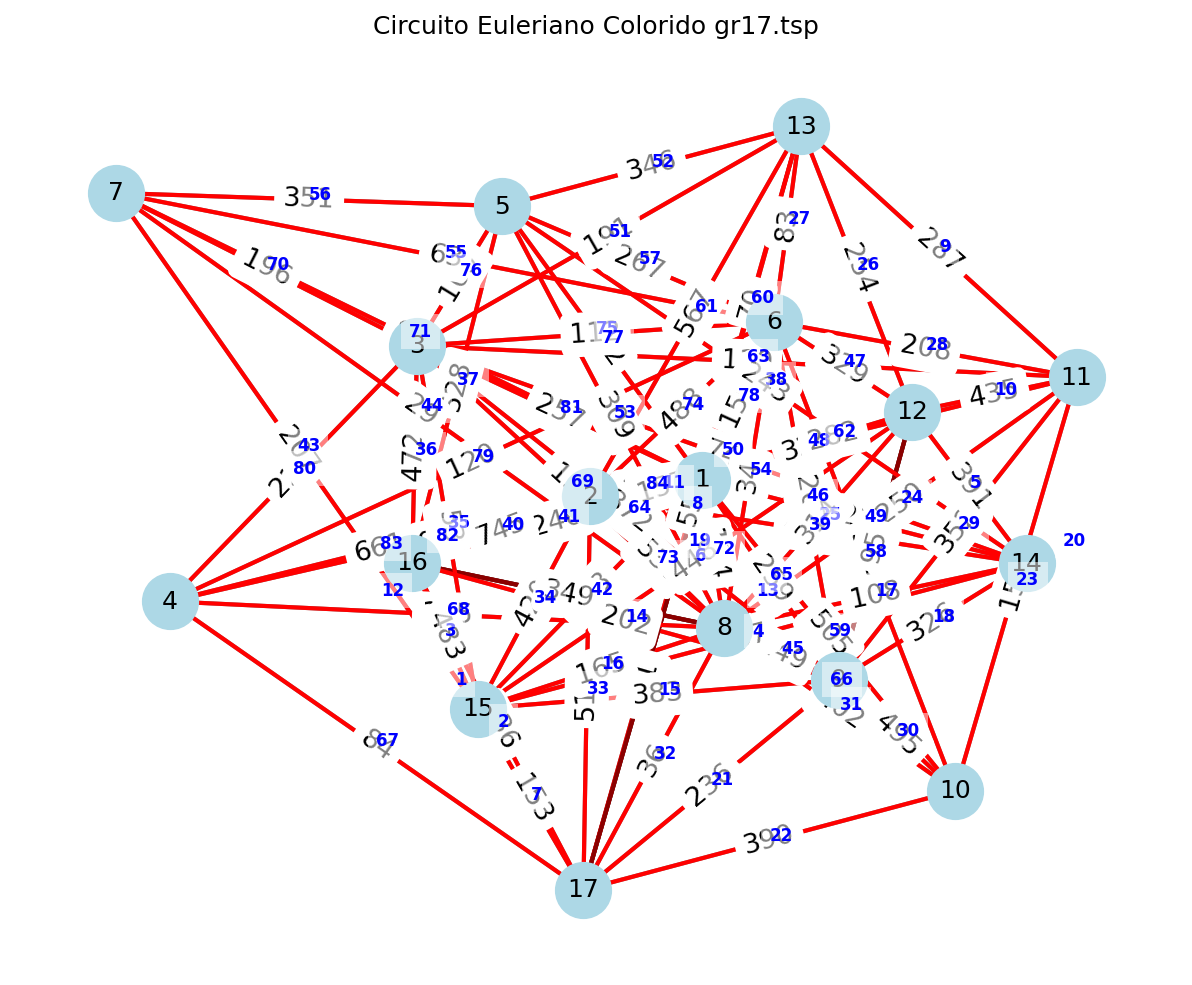
\includegraphics[width=0.6\textwidth]{./resultado/circuito_euleriano_gr17.tsp.png}
    \caption{Circuito euleriano encontrado para a instância gr17.tsp}
    \label{fig:circuito_euleriano_gr17}
\end{figure}

O percurso apresentado na tabela corresponde ao caminho percorrido no circuito euleriano da instância gr17.tsp, garantindo que todas as arestas do grafo sejam visitadas ao menos uma vez com o menor custo total possível. As imagens e a tabela permitem validar visualmente e numericamente a solução encontrada pelo algoritmo para um grafo de maior complexidade.

\subsection{Análise da instância gr21.tsp}

A instância gr21.tsp consiste em um grafo com 21 vértices, baseado em problemas clássicos de roteamento, com distâncias fornecidas em formato de matriz triangular inferior. Essa instância exige tratamento específico na leitura dos dados e permite avaliar o algoritmo em cenários ainda mais complexos.

\noindent A Figura~\ref{fig:grafo_gr21} apresenta o grafo original da instância gr21.tsp. O percurso ótimo está detalhado na Tabela~\ref{tab:percurso_gr21} e ilustrado na Figura~\ref{fig:circuito_euleriano_gr21}.

\begin{figure}[H]
    \centering
    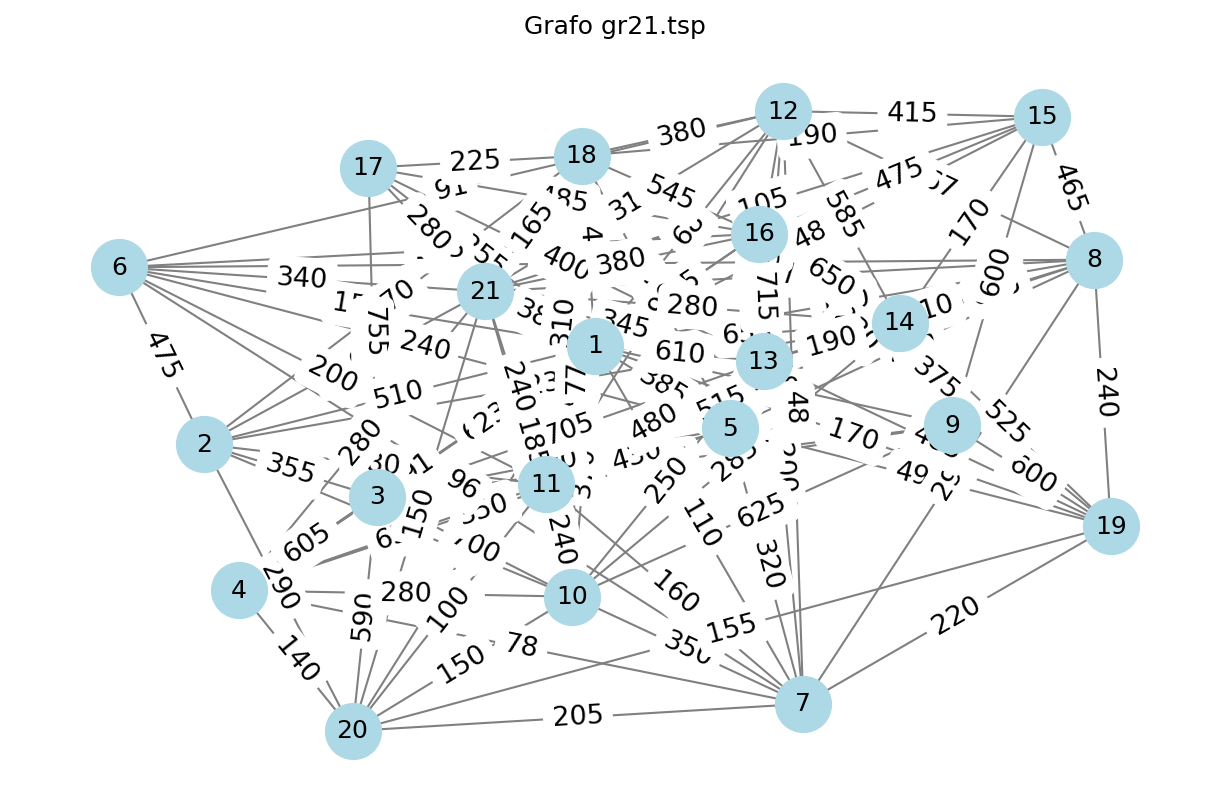
\includegraphics[width=0.6\textwidth]{./resultado/grafo_gr21.tsp.png}
    \caption{Grafo original da instância gr21.tsp}
    \label{fig:grafo_gr21}
\end{figure}

\textbf{Resultados obtidos:}
\begin{itemize}
    \item Dimensão (Vértices): 21
    \item Arestas Originais: 113
    \item Custo Original: 38429
    \item Custo Final: 39823
    \item Vértices de Grau Ímpar: 10
    \item Arestas Duplicadas: 5
    \item Overhead: 1394 (3.63\%)
\end{itemize}

\begin{table}[H]
    \centering
    \scriptsize
    \begin{tabular}{|c|c|c|c|c|}
        \hline
        \multicolumn{5}{|c|}{Percurso} \\ \hline
    1 -- (380) $\rightarrow$ 21 & 21 -- (165) $\rightarrow$ 18 & 18 -- (225) $\rightarrow$ 17 & 17 -- (280) $\rightarrow$ 21 & 21 -- (150) $\rightarrow$ 20 \\
    20 -- (155) $\rightarrow$ 19 & 19 -- (375) $\rightarrow$ 16 & 16 -- (380) $\rightarrow$ 21 & 21 -- (280) $\rightarrow$ 14 & 14 -- (525) $\rightarrow$ 19 \\
    19 -- (485) $\rightarrow$ 13 & 13 -- (345) $\rightarrow$ 21 & 21 -- (240) $\rightarrow$ 11 & 11 -- (100) $\rightarrow$ 20 & 20 -- (150) $\rightarrow$ 10 \\
    10 -- (185) $\rightarrow$ 21 & 21 -- (105) $\rightarrow$ 15 & 15 -- (190) $\rightarrow$ 18 & 18 -- (545) $\rightarrow$ 16 & 16 -- (475) $\rightarrow$ 15 \\
    15 -- (170) $\rightarrow$ 14 & 14 -- (650) $\rightarrow$ 16 & 16 -- (485) $\rightarrow$ 17 & 17 -- (400) $\rightarrow$ 13 & 13 -- (715) $\rightarrow$ 16 \\
    16 -- (230) $\rightarrow$ 9 & 9 -- (600) $\rightarrow$ 19 & 19 -- (240) $\rightarrow$ 8 & 8 -- (370) $\rightarrow$ 21 & 21 -- (310) $\rightarrow$ 12 \\
    12 -- (585) $\rightarrow$ 14 & 14 -- (190) $\rightarrow$ 13 & 13 -- (545) $\rightarrow$ 12 & 12 -- (380) $\rightarrow$ 18 & 18 -- (310) $\rightarrow$ 11 \\
    11 -- (515) $\rightarrow$ 14 & 14 -- (285) $\rightarrow$ 10 & 10 -- (250) $\rightarrow$ 13 & 13 -- (480) $\rightarrow$ 11 & 11 -- (240) $\rightarrow$ 10 \\
    10 -- (77) $\rightarrow$ 18 & 18 -- (660) $\rightarrow$ 5 & \textcolor{red}{5 -- (495) $\rightarrow$ 19} & 19 -- (220) $\rightarrow$ 7 & 7 -- (205) $\rightarrow$ 20 \\
    \textcolor{red}{20 -- (590) $\rightarrow$ 3} & \textcolor{red}{3 -- (590) $\rightarrow$ 20} & 20 -- (140) $\rightarrow$ 4 & 4 -- (280) $\rightarrow$ 21 & \textcolor{red}{21 -- (140) $\rightarrow$ 2} \\
    \textcolor{red}{2 -- (140) $\rightarrow$ 21} & 21 -- (340) $\rightarrow$ 6 & 6 -- (125) $\rightarrow$ 16 & 16 -- (200) $\rightarrow$ 7 & 7 -- (160) $\rightarrow$ 11 \\
    11 -- (90) $\rightarrow$ 12 & 12 -- (415) $\rightarrow$ 15 & 15 -- (600) $\rightarrow$ 9 & 9 -- (775) $\rightarrow$ 14 & 14 -- (645) $\rightarrow$ 8 \\
    8 -- (610) $\rightarrow$ 13 & 13 -- (835) $\rightarrow$ 5 & \textcolor{red}{5 -- (495) $\rightarrow$ 19} & 19 -- (170) $\rightarrow$ 1 & 1 -- (240) $\rightarrow$ 20 \\
    20 -- (290) $\rightarrow$ 2 & 2 -- (270) $\rightarrow$ 18 & 18 -- (450) $\rightarrow$ 1 & 1 -- (265) $\rightarrow$ 16 & 16 -- (235) $\rightarrow$ 4 \\
    4 -- (63) $\rightarrow$ 11 & 11 -- (535) $\rightarrow$ 9 & 9 -- (625) $\rightarrow$ 10 & 10 -- (350) $\rightarrow$ 7 & 7 -- (48) $\rightarrow$ 12 \\
    \textcolor{red}{12 -- (91) $\rightarrow$ 6} & \textcolor{red}{6 -- (91) $\rightarrow$ 12} & 12 -- (67) $\rightarrow$ 8 & 8 -- (465) $\rightarrow$ 15 & 15 -- (480) $\rightarrow$ 1 \\
    1 -- (255) $\rightarrow$ 17 & 17 -- (755) $\rightarrow$ 3 & 3 -- (705) $\rightarrow$ 13 & 13 -- (610) $\rightarrow$ 1 & 1 -- (655) $\rightarrow$ 14 \\
    14 -- (235) $\rightarrow$ 2 & 2 -- (380) $\rightarrow$ 11 & 11 -- (430) $\rightarrow$ 5 & 5 -- (320) $\rightarrow$ 12 & 12 -- (68) $\rightarrow$ 1 \\
    1 -- (155) $\rightarrow$ 11 & 11 -- (200) $\rightarrow$ 6 & 6 -- (36) $\rightarrow$ 8 & 8 -- (29) $\rightarrow$ 7 & 7 -- (320) $\rightarrow$ 5 \\
    5 -- (285) $\rightarrow$ 8 & 8 -- (130) $\rightarrow$ 1 & 1 -- (490) $\rightarrow$ 9 & 9 -- (295) $\rightarrow$ 3 & 3 -- (700) $\rightarrow$ 10 \\
    10 -- (280) $\rightarrow$ 4 & \textcolor{red}{4 -- (78) $\rightarrow$ 7} & 7 -- (96) $\rightarrow$ 6 & 6 -- (240) $\rightarrow$ 5 & 5 -- (350) $\rightarrow$ 4 \\
    \textcolor{red}{4 -- (78) $\rightarrow$ 7} & 7 -- (110) $\rightarrow$ 1 & 1 -- (370) $\rightarrow$ 10 & 10 -- (320) $\rightarrow$ 2 & 2 -- (475) $\rightarrow$ 6 \\
    6 -- (155) $\rightarrow$ 1 & 1 -- (385) $\rightarrow$ 5 & 5 -- (390) $\rightarrow$ 3 & 3 -- (605) $\rightarrow$ 4 & 4 -- (91) $\rightarrow$ 1 \\
    1 -- (635) $\rightarrow$ 3 & 3 -- (355) $\rightarrow$ 2 & 2 -- (510) $\rightarrow$ 1 &   &   \\
        \hline
    \end{tabular}
    \caption{Percurso ótimo encontrado para a Instância gr21.tsp. Células em vermelho indicam arestas emparelhadas pelo algoritmo.}
    \label{tab:percurso_gr21}
\end{table}



\begin{figure}[H]
    \centering
    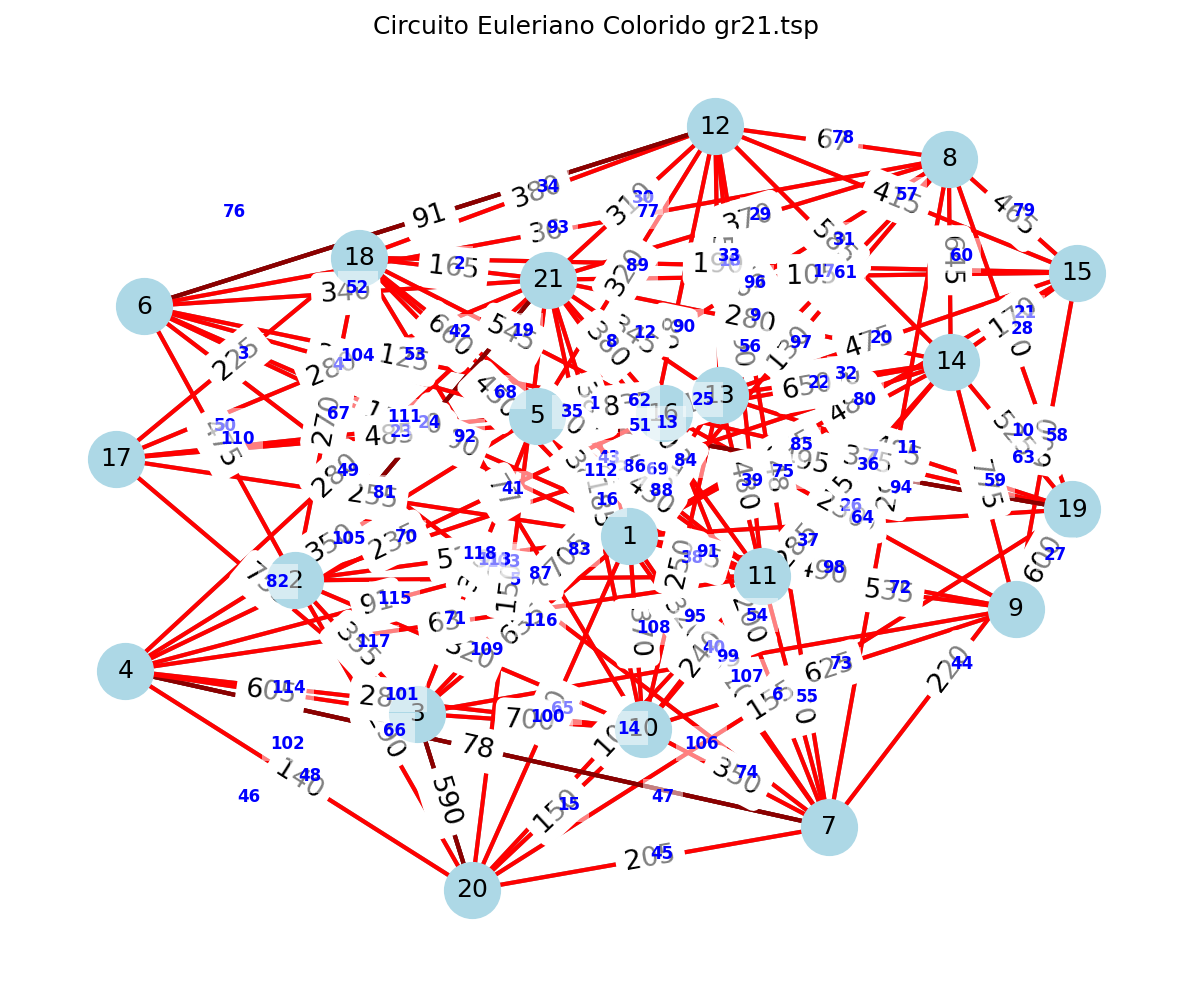
\includegraphics[width=0.6\textwidth]{./resultado/circuito_euleriano_gr21.tsp.png}
    \caption{Circuito euleriano encontrado para a instância gr21.tsp}
    \label{fig:circuito_euleriano_gr21}
\end{figure}

O percurso apresentado na tabela corresponde ao caminho percorrido no circuito euleriano da instância gr21.tsp, garantindo que todas as arestas do grafo sejam visitadas ao menos uma vez com o menor custo total possível. As imagens e a tabela permitem validar visualmente e numericamente a solução encontrada pelo algoritmo para um grafo de porte elevado.

\subsection{Análise da instância gr24.tsp}

A instância gr24.tsp consiste em um grafo com 24 vértices e distâncias explícitas entre pares de cidades. É a maior instância utilizada neste trabalho, permitindo avaliar o desempenho do algoritmo em cenários próximos de aplicações reais, com grande número de vértices e arestas.

\noindent A Figura~\ref{fig:grafo_gr24} apresenta o grafo original da instância gr24.tsp. O percurso ótimo está detalhado na Tabela~\ref{tab:percurso_gr24} e ilustrado na Figura~\ref{fig:circuito_euleriano_gr24}.

\begin{figure}[H]
    \centering
    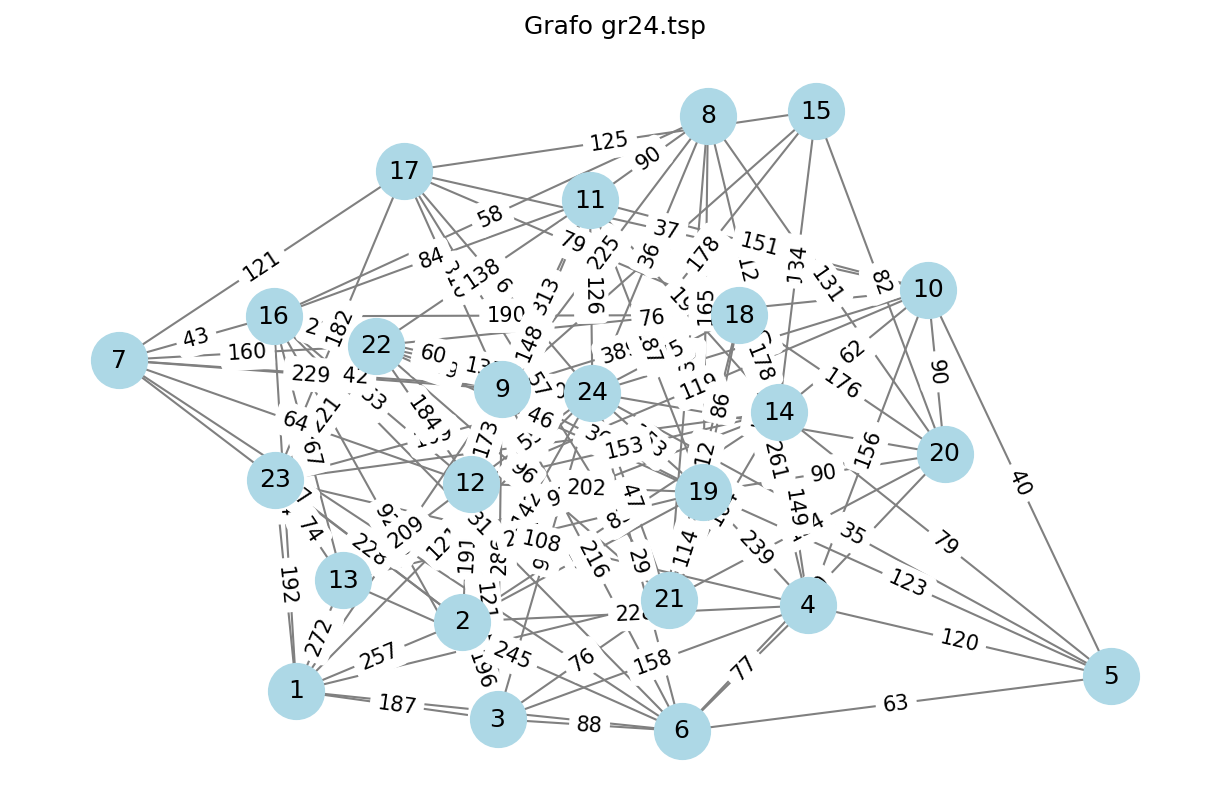
\includegraphics[width=0.6\textwidth]{./resultado/grafo_gr24.tsp.png}
    \caption{Grafo original da instância gr24.tsp}
    \label{fig:grafo_gr24}
\end{figure}

\textbf{Resultados obtidos:}
\begin{itemize}
    \item Dimensão (Vértices): 24
    \item Arestas Originais: 116
    \item Custo Original: 16541
    \item Custo Final: 17678
    \item Vértices de Grau Ímpar: 12
    \item Arestas Duplicadas: 6
    \item Overhead: 1137 (6.87\%)
\end{itemize}

\begin{table}[H]
    \centering
    \scriptsize
    \begin{tabular}{|c|c|c|c|c|}
        \hline
        \multicolumn{5}{|c|}{Percurso} \\ \hline
    1 -- (121) $\rightarrow$ 24 & 24 -- (146) $\rightarrow$ 20 & 20 -- (82) $\rightarrow$ 15 & 15 -- (125) $\rightarrow$ 17 & 17 -- (79) $\rightarrow$ 18 \\
    18 -- (176) $\rightarrow$ 20 & 20 -- (131) $\rightarrow$ 8 & 8 -- (90) $\rightarrow$ 11 & 11 -- (138) $\rightarrow$ 22 & 22 -- (76) $\rightarrow$ 10 \\
    10 -- (90) $\rightarrow$ 20 & 20 -- (90) $\rightarrow$ 19 & 19 -- (46) $\rightarrow$ 22 & 22 -- (160) $\rightarrow$ 7 & 7 -- (121) $\rightarrow$ 17 \\
    17 -- (37) $\rightarrow$ 10 & \textcolor{red}{10 -- (151) $\rightarrow$ 11} & \textcolor{red}{11 -- (151) $\rightarrow$ 10} & 10 -- (40) $\rightarrow$ 5 & 5 -- (123) $\rightarrow$ 19 \\
    19 -- (86) $\rightarrow$ 18 & \textcolor{red}{18 -- (261) $\rightarrow$ 4} & \textcolor{red}{4 -- (261) $\rightarrow$ 18} & 18 -- (178) $\rightarrow$ 14 & 14 -- (134) $\rightarrow$ 15 \\
    15 -- (178) $\rightarrow$ 24 & 24 -- (135) $\rightarrow$ 22 & 22 -- (184) $\rightarrow$ 12 & 12 -- (202) $\rightarrow$ 19 & 19 -- (187) $\rightarrow$ 11 \\
    11 -- (199) $\rightarrow$ 14 & 14 -- (62) $\rightarrow$ 10 & 10 -- (156) $\rightarrow$ 4 & 4 -- (239) $\rightarrow$ 19 & 19 -- (165) $\rightarrow$ 8 \\
    8 -- (112) $\rightarrow$ 14 & 14 -- (79) $\rightarrow$ 5 & 5 -- (120) $\rightarrow$ 4 & 4 -- (149) $\rightarrow$ 14 & 14 -- (153) $\rightarrow$ 12 \\
    12 -- (148) $\rightarrow$ 11 & 11 -- (126) $\rightarrow$ 24 & 24 -- (70) $\rightarrow$ 10 & 10 -- (119) $\rightarrow$ 12 & 12 -- (64) $\rightarrow$ 7 \\
    7 -- (42) $\rightarrow$ 24 & 24 -- (153) $\rightarrow$ 19 & 19 -- (114) $\rightarrow$ 21 & 21 -- (96) $\rightarrow$ 22 & 22 -- (221) $\rightarrow$ 23 \\
    23 -- (169) $\rightarrow$ 24 & 24 -- (175) $\rightarrow$ 18 & 18 -- (190) $\rightarrow$ 16 & 16 -- (212) $\rightarrow$ 22 & 22 -- (349) $\rightarrow$ 9 \\
    9 -- (389) $\rightarrow$ 18 & 18 -- (112) $\rightarrow$ 21 & 21 -- (47) $\rightarrow$ 24 & 24 -- (55) $\rightarrow$ 12 & 12 -- (53) $\rightarrow$ 16 \\
    16 -- (60) $\rightarrow$ 24 & 24 -- (96) $\rightarrow$ 17 & 17 -- (182) $\rightarrow$ 23 & 23 -- (96) $\rightarrow$ 14 & 14 -- (104) $\rightarrow$ 21 \\
    21 -- (57) $\rightarrow$ 17 & 17 -- (310) $\rightarrow$ 9 & \textcolor{red}{9 -- (248) $\rightarrow$ 15} & \textcolor{red}{15 -- (248) $\rightarrow$ 9} & 9 -- (220) $\rightarrow$ 24 \\
    24 -- (36) $\rightarrow$ 8 & 8 -- (58) $\rightarrow$ 16 & 16 -- (84) $\rightarrow$ 11 & 11 -- (313) $\rightarrow$ 9 & 9 -- (367) $\rightarrow$ 19 \\
    \textcolor{red}{19 -- (227) $\rightarrow$ 13} & 13 -- (74) $\rightarrow$ 23 & 23 -- (228) $\rightarrow$ 2 & 2 -- (53) $\rightarrow$ 19 & \textcolor{red}{19 -- (227) $\rightarrow$ 13} \\
    13 -- (267) $\rightarrow$ 16 & 16 -- (43) $\rightarrow$ 7 & 7 -- (229) $\rightarrow$ 9 & 9 -- (225) $\rightarrow$ 8 & 8 -- (30) $\rightarrow$ 21 \\
    21 -- (134) $\rightarrow$ 20 & 20 -- (200) $\rightarrow$ 6 & 6 -- (29) $\rightarrow$ 24 & 24 -- (99) $\rightarrow$ 3 & 3 -- (92) $\rightarrow$ 16 \\
    16 -- (31) $\rightarrow$ 6 & 6 -- (216) $\rightarrow$ 9 & 9 -- (173) $\rightarrow$ 12 & 12 -- (209) $\rightarrow$ 13 & 13 -- (97) $\rightarrow$ 14 \\
    14 -- (83) $\rightarrow$ 2 & 2 -- (142) $\rightarrow$ 24 & 24 -- (35) $\rightarrow$ 5 & 5 -- (63) $\rightarrow$ 6 & 6 -- (25) $\rightarrow$ 7 \\
    7 -- (167) $\rightarrow$ 2 & 2 -- (191) $\rightarrow$ 12 & 12 -- (121) $\rightarrow$ 3 & 3 -- (76) $\rightarrow$ 21 & 21 -- (175) $\rightarrow$ 1 \\
    \textcolor{red}{1 -- (54) $\rightarrow$ 16} & \textcolor{red}{16 -- (54) $\rightarrow$ 1} & 1 -- (192) $\rightarrow$ 23 & 23 -- (108) $\rightarrow$ 4 & 4 -- (77) $\rightarrow$ 6 \\
    6 -- (245) $\rightarrow$ 13 & 13 -- (272) $\rightarrow$ 1 & 1 -- (243) $\rightarrow$ 9 & 9 -- (286) $\rightarrow$ 3 & 3 -- (158) $\rightarrow$ 4 \\
    4 -- (228) $\rightarrow$ 2 & \textcolor{red}{2 -- (196) $\rightarrow$ 3} & 3 -- (88) $\rightarrow$ 6 & 6 -- (80) $\rightarrow$ 1 & 1 -- (187) $\rightarrow$ 3 \\
    \textcolor{red}{3 -- (196) $\rightarrow$ 2} & 2 -- (257) $\rightarrow$ 1 &   &   &   \\
        \hline
    \end{tabular}
    \caption{Percurso ótimo encontrado para a Instância gr24.tsp. Células em vermelho indicam arestas emparelhadas pelo algoritmo.}
    \label{tab:percurso_gr24}
\end{table}



\begin{figure}[H]
    \centering
    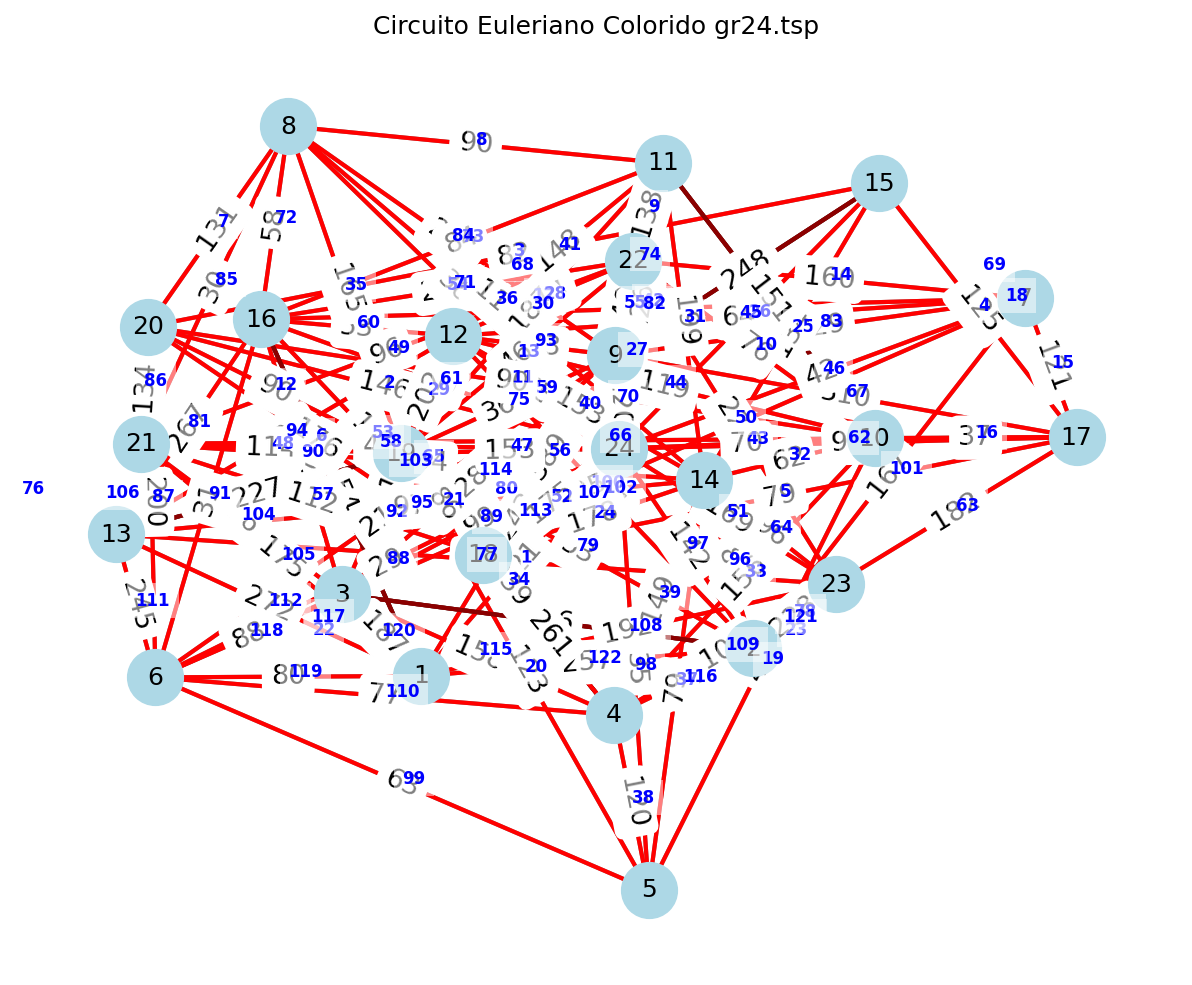
\includegraphics[width=0.6\textwidth]{./resultado/circuito_euleriano_gr24.tsp.png}
    \caption{Circuito euleriano encontrado para a instância gr24.tsp}
    \label{fig:circuito_euleriano_gr24}
\end{figure}

O percurso apresentado na tabela corresponde ao caminho percorrido no circuito euleriano da instância gr24.tsp, garantindo que todas as arestas do grafo sejam visitadas ao menos uma vez com o menor custo total possível. As imagens e a tabela permitem validar visualmente e numericamente a solução encontrada pelo algoritmo para um grafo de grande porte.

\section{Conclusão}

O algoritmo implementado resolve eficientemente o Problema do Caixeiro Chinês através de uma abordagem estruturada em três etapas fundamentais: (i) identificação de vértices com grau ímpar e cálculo de caminhos mínimos entre eles via algoritmo de Dijkstra; (ii) emparelhamento ótimo desses vértices, duplicando as arestas de menor custo para eulerizar o grafo; e (iii) construção do circuito euleriano utilizando o algoritmo de Hierholzer. Esta estratégia garante que todas as arestas sejam percorridas ao menos uma vez com custo total mínimo.

Os testes realizados em cinco instâncias de complexidade crescente (7, 15, 17, 21 e 24 vértices) demonstram a robustez e escalabilidade do algoritmo. A instância de teste validou a correção da implementação com overhead de 31.94\%, onde 2 arestas foram duplicadas dentre 10 originais. As instâncias intermediárias (15 e 17 vértices) apresentaram overheads de 12.51\% e 2.56\%, respectivamente, demonstrando melhoria proporcional da qualidade das soluções com o crescimento do tamanho do grafo. As instâncias de grande porte (21 e 24 vértices) exibiram overheads de 3.63\% e 6.87\%, consolidando a eficiência da abordagem em cenários de maior complexidade.

A Tabela~\ref{tab:resumo_resultados} sintetiza todos os resultados obtidos:

\begin{table}[H]
    \centering
    \footnotesize
    \begin{tabular}{|l|c|c|c|c|c|c|c|c|}
        \hline
        \textbf{Inst.} & \textbf{Dim} & \textbf{Arestas} & \textbf{C. Orig.} & \textbf{C. Final} & \textbf{V. Ím.} & \textbf{A. Dup.} & \textbf{Overhead} & \textbf{O. \%} \\ \hline
        aula.tsp & 7 & 10 & 72 & 95 & 4 & 2 & 23 & 31.94\% \\ \hline
        gr15.tsp & 15 & 40 & 1871 & 2105 & 8 & 4 & 234 & 12.51\% \\ \hline
        gr17.tsp & 17 & 81 & 22061 & 22626 & 6 & 3 & 565 & 2.56\% \\ \hline
        gr21.tsp & 21 & 113 & 38429 & 39823 & 10 & 5 & 1394 & 3.63\% \\ \hline
        gr24.tsp & 24 & 116 & 16541 & 17678 & 12 & 6 & 1137 & 6.87\% \\ \hline
    \end{tabular}
    \caption{Resumo integrado dos resultados: dimensão do grafo, arestas originais, custos original e final, vértices de grau ímpar, arestas duplicadas e overhead em valor absoluto e percentual.}
    \label{tab:resumo_resultados}
\end{table}


Durante o desenvolvimento, foi possível compreender empiricamente como a distribuição e a quantidade de vértices de grau ímpar influenciam diretamente o custo adicional necessário para eulerizar o grafo. A análise dos dados revela padrões significativos: instâncias com mais vértices tendem a apresentar overheads percentuais menores, sugerindo que em grafos maiores, o impacto relativo da eulerização diminui. Essa observação é importante para aplicações de roteamento e otimização logística em larga escala, onde o algoritmo demonstra potencial de aplicação prática.

O trabalho contribuiu para consolidar conceitos fundamentais da teoria dos grafos, particularmente o Teorema de Euler e suas condições de aplicabilidade, a relevância do emparelhamento de peso mínimo na construção de soluções ótimas e a eficiência computacional dos algoritmos de caminhos mínimos e circuitos eulerianos. Sob a perspectiva prática, a implementação fornece uma ferramenta viável para problemas reais de roteamento, tais como planejamento de rotas de entrega, inspeção de redes de infraestrutura e coleta de resíduos urbanos, onde é necessário percorrer todas as vias pelo menos uma vez com custo mínimo. A escalabilidade demonstrada em instâncias com até 24 vértices indica potencial para extensão a problemas de maior magnitude.

A implementação alcançou seus objetivos de desenvolver um algoritmo eficiente, testá-lo em múltiplas instâncias e validar a correção das soluções obtidas. O código modular permitiu flexibilidade na manipulação de diferentes formatos de entrada e na geração de visualizações detalhadas dos percursos e grafos eulerianos. Recomenda-se para trabalhos futuros a investigação de otimizações heurísticas para instâncias de escala muito maior e a comparação com outras abordagens metaheurísticas para validação empírica de otimalidade.


\section{Referências}
\bibliography{referencias}
\bibliographystyle{abntex2-alf}
\end{document}
